\chapter{Introduction}\label{chap:intro}

\section{Problem statement}

The Wireless Sensor Networks (WSNs) have recently emerged as a promising computing platform for many nontraditional applications, such as wildfire monitoring in the forest, wildlife tracing in the deep ocean, and intelligence surveillance in the battle field. A WSN usually consists of hundreds of sensor nodes that are equipped with the sensors to measure the physical phenomena, such as temperature, humidity, pressure, or movement of objects. Sensing results are constructed into data packets and routed back to sink nodes, which are typically more powerful, user accessible and have fewer energy constrains.

\begin{figure}[h]
\centering
\mbox{\subfigure[Mica2 sensor]{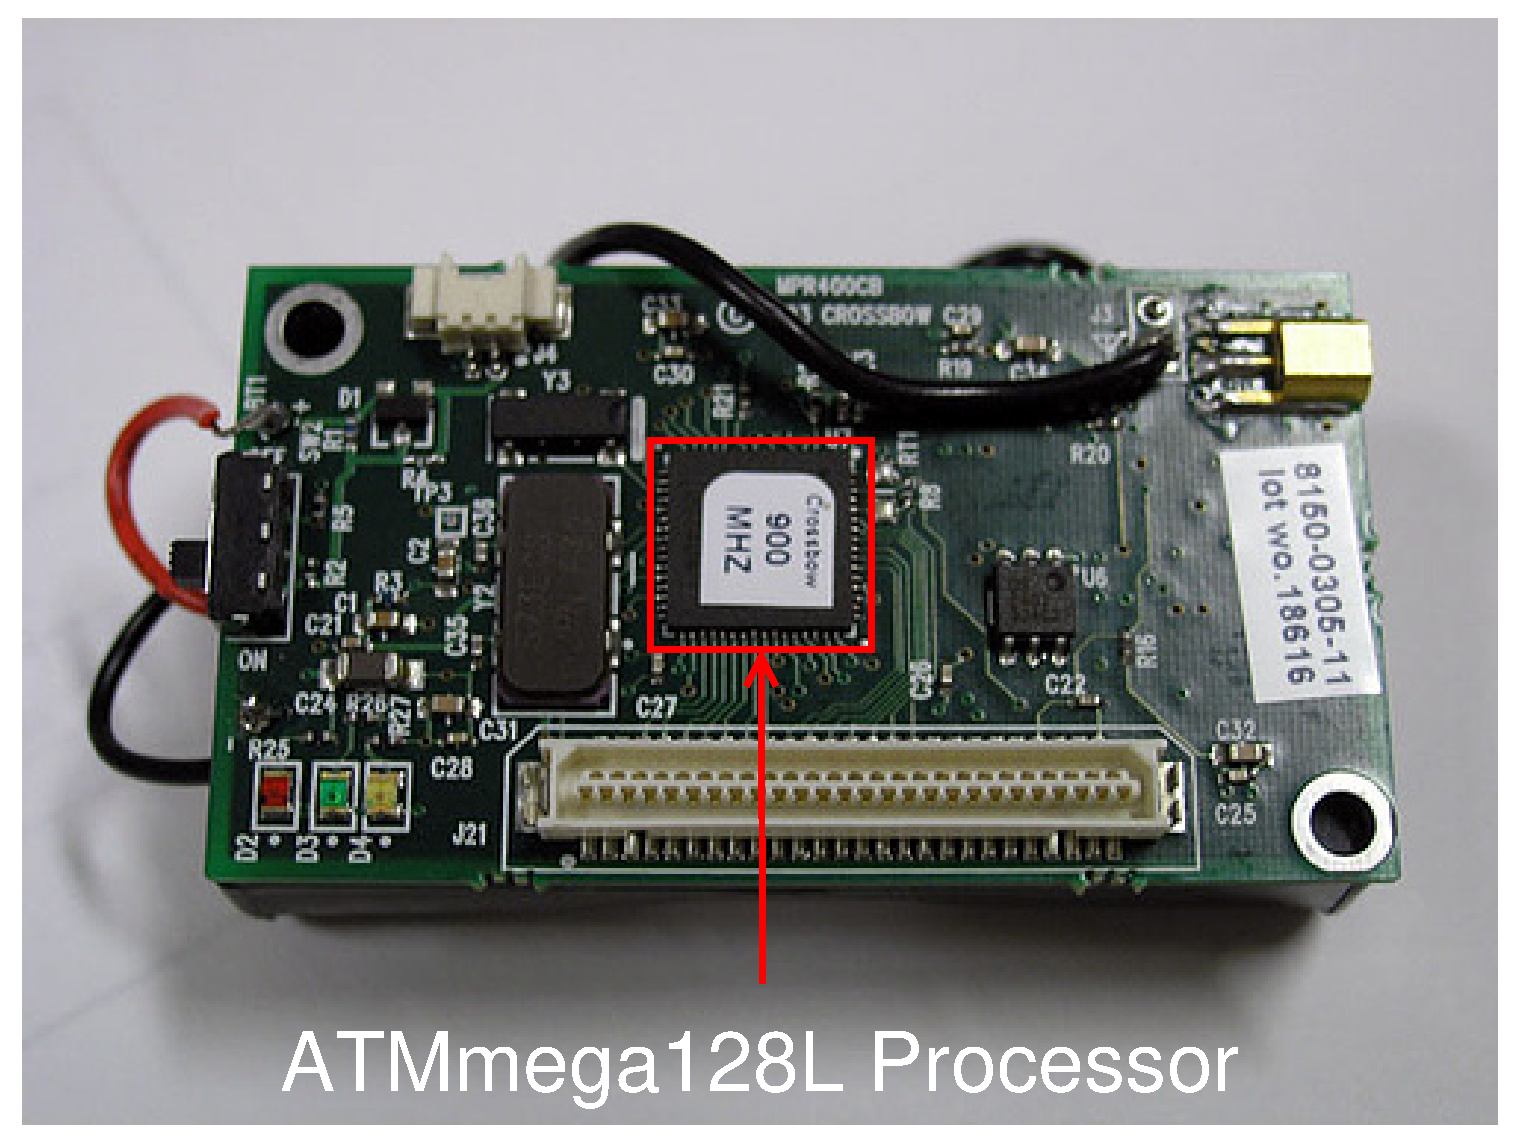
\includegraphics[width=2in]{figures/mica2.eps}}\quad
     \subfigure[Mica2 block diagram]{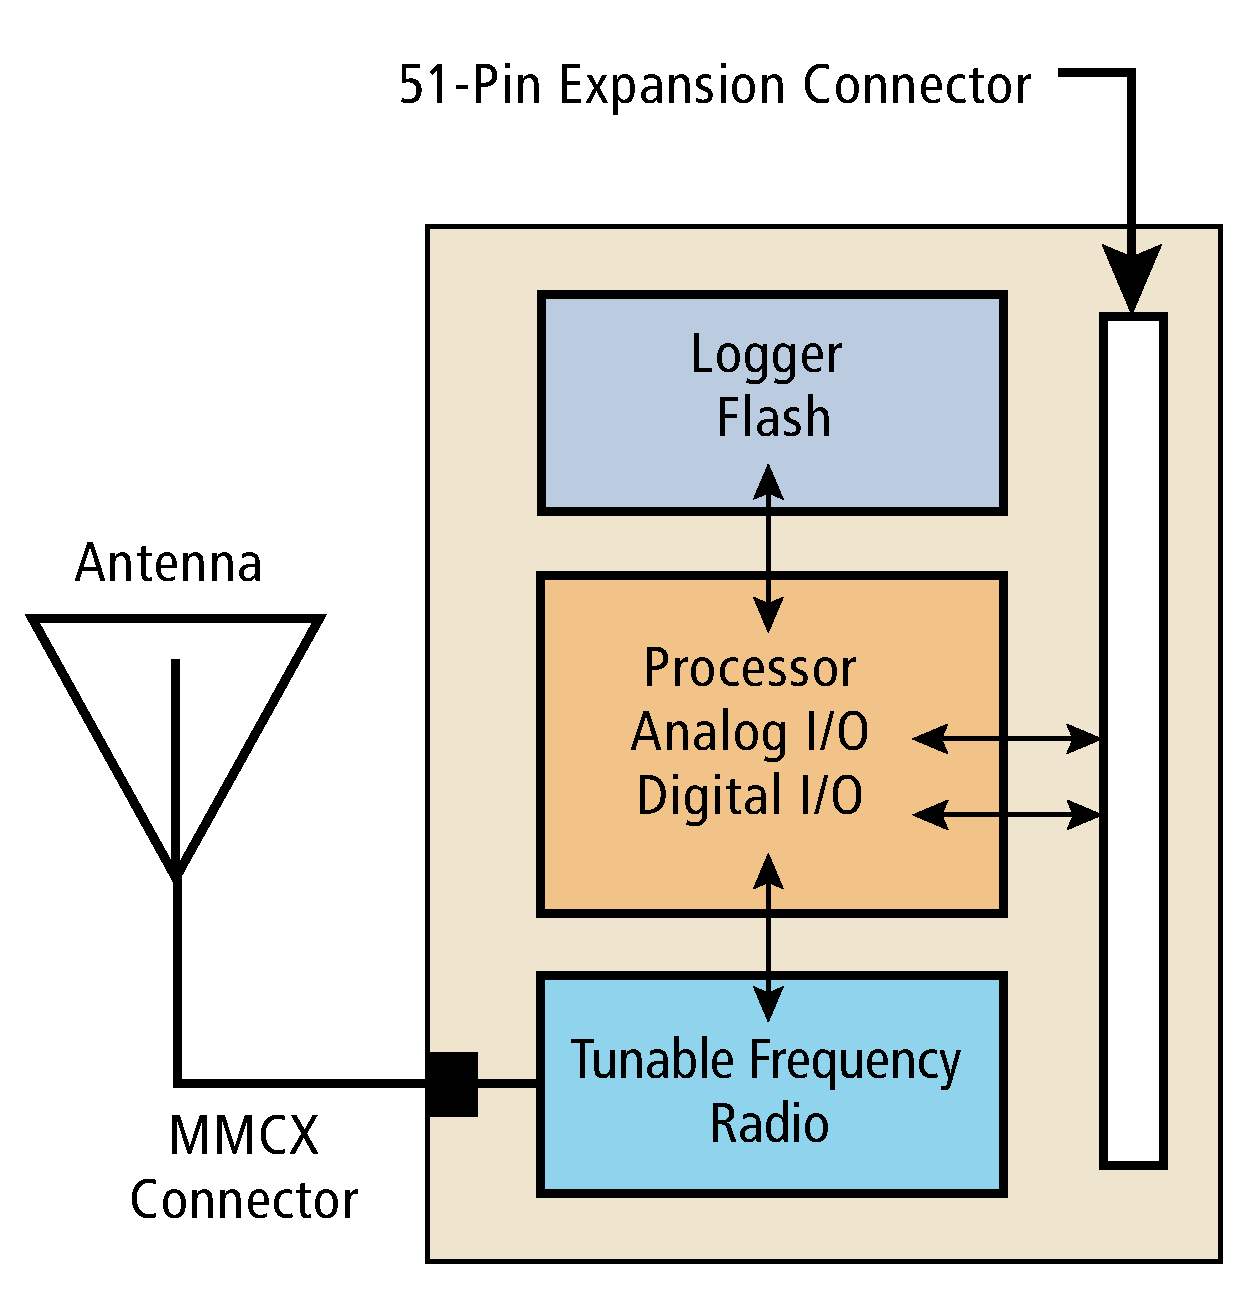
\includegraphics[width=2in]{figures/mpr400.eps}}\quad}
\caption{Mica2 and block diagram.}
\label{fig:mica2}
\end{figure}

The sensor nodes are mainly equipped with processors, sensing devices and communication transceivers. Because they get limited power supplies from the batteries, the simple sensor nodes~\cite{mica2-power, micaz-power,telos,telosb} are equipped with single low power consumption processor. 
For example, a Mica2~\cite{mica2-power} mote shown in Figure~\ref{fig:mica2}, is equipped with a 8MHz ATmega128L processor to process the sensed data.

With technology advances, sensors equipped with multiple chips~\cite{imote2} have been proposed recently. Imote2~\cite{imote2} developed by Intel includes a DSP chip on the mote besides the CPU core to support image and video operations, shown in Figure~\ref{fig:imote2}. So that the multi-chip sensors can furthermore process the multimedia content sensed by the equipped camera and microphones in order to reduce the number of data packets that need to be transmitted to the sink node.

\begin{figure}[h]
\centering
\mbox{\subfigure[Imote2 sensor]{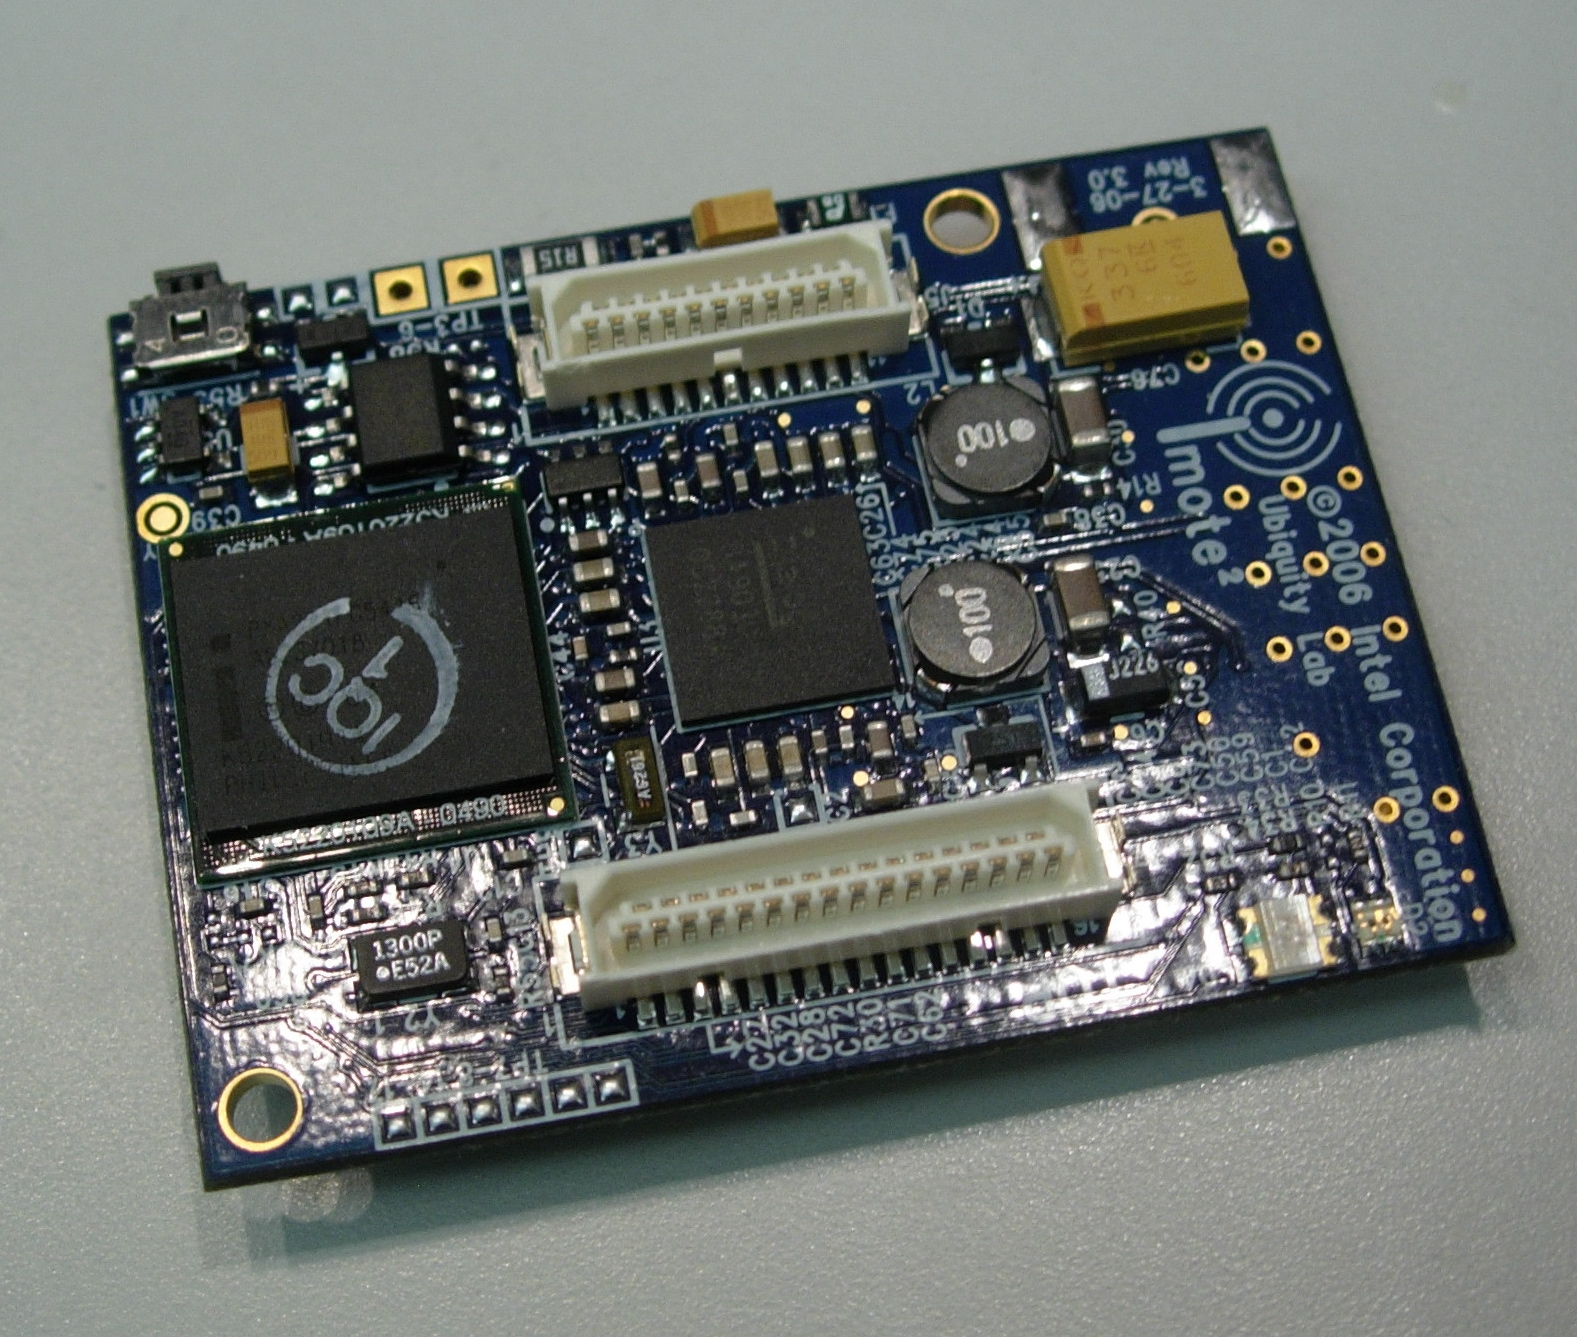
\includegraphics[width=2.2in]{figures/imote2.eps}}\quad
      \subfigure[Imote2 block diagram]{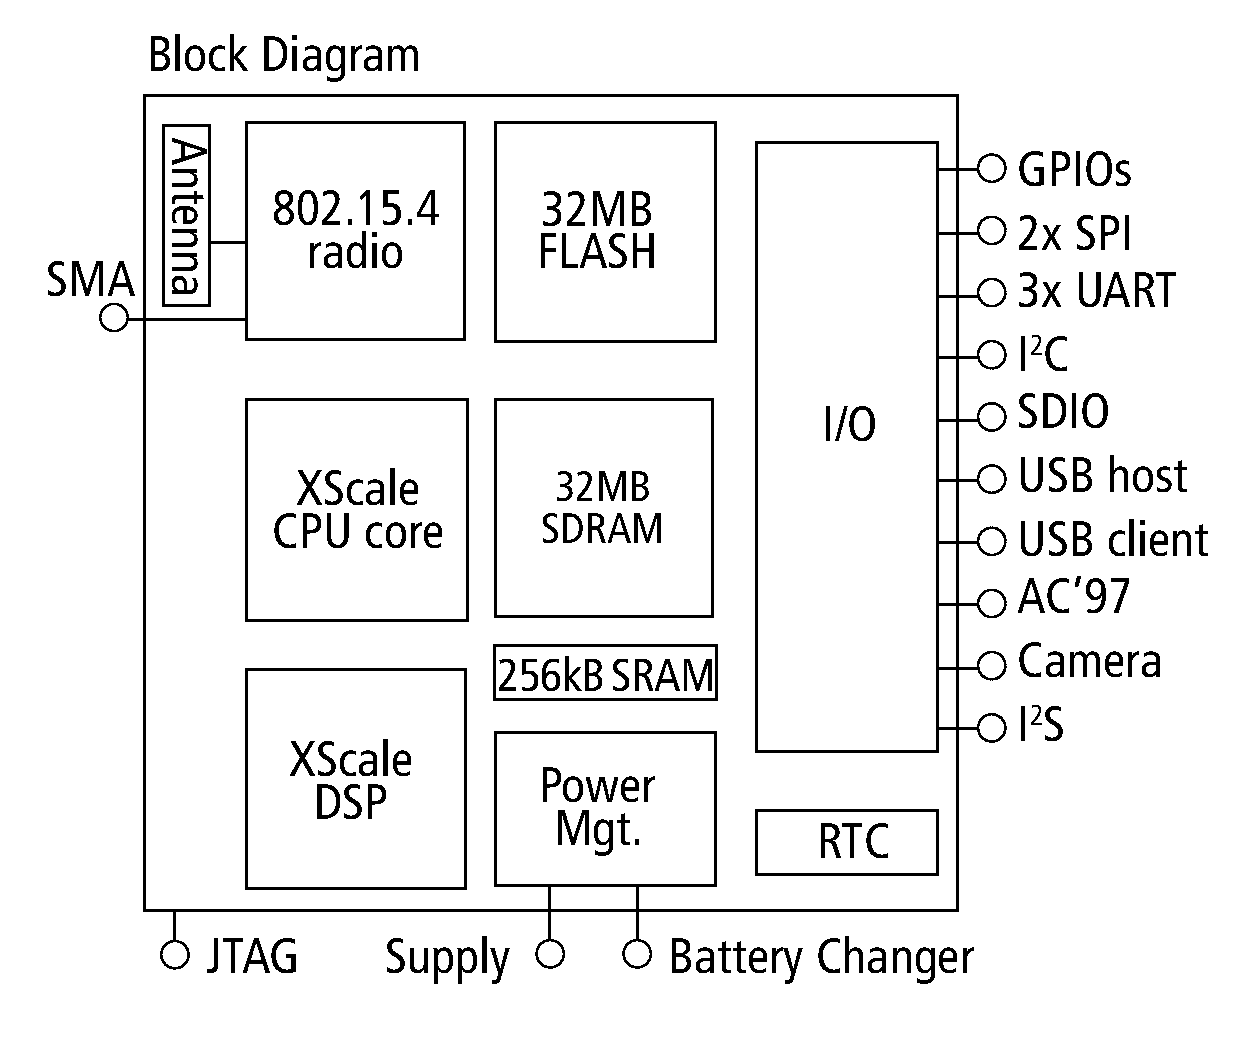
\includegraphics[width=2.2in]{figures/imotedia.eps}}\quad}
\caption{Imote2 sensor and block diagram.}
\label{fig:imote2}
\end{figure}

The multi-chip sensor design brings a lot of design opportunities into WSN study. The high manufacture cost of these sensor nodes makes it economically less appealing to let the whole network run just one application. Recently, researchers have envisioned the wide adoption of multi-application WSNs (MA-WSNs), which can support several applications in one network infrastructure~\cite{melete,ma-wsns}. Besides the concurrent application execution in one network, MA-WSNs can also let one sensor node execute different applications at different time period.
The sensors store the code of multiple applications in the external flash memory and load the selected application into the program memory for the desired functionality.

Compared to single-application WSNs (SA-WSNs), MA-WSNs have many advantages. For example, MA-WSN can be deployed in a national park to monitor both wildfires and animal movement. More sensors can be set to monitor the animal movement in the early morning or late afternoon when animals tend to leave from or return to their habinates; and more sensors could be set to monitor wildfires in the summer season when the chance to catch fires is high. By exploiting the same network infrastructure for both events, (1) MA-WSNs save the investment and effort in deploying and testing two sensor networks; (2) the sensor network adapts better to the dynamic changing environment and even adjusts the coverage according to the need.

In both SA-WSNs and MA-WSNs, the application(s) running on the sensors may need to fix bugs or add new features, after the deployment. For example, the WSN may be deployed in an area which human beings are not familiar with. After the sensor nodes are deployed, data will be collected and sent back to the sink node. With more knowledge about the environment, the scientists may be able to adjust the sensing functions to make them more accurate based on the preliminary data analysis. I formulate updating code or data of a running application in the network as the software upgrade problem in WSN software update. As shown in Figure~\ref{fig:upgrade}, software upgrade involves binary code generation on the sink node, the routing design of the update binary patches to the target sensor nodes and the image replacement on the sensor nodes.

\begin{figure}[htbp]
	\centering
		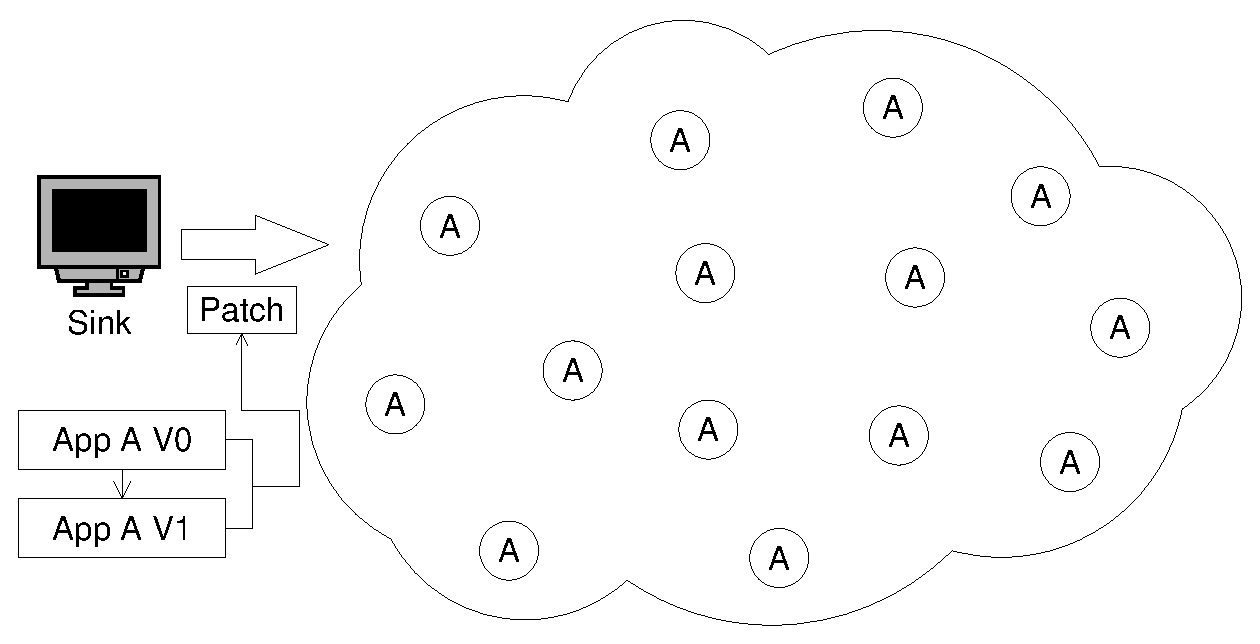
\includegraphics[scale=0.35]{figures/upgrade.eps}
	\caption{Software upgrade.}
	\label{fig:upgrade}
\end{figure}

Besides software upgrade, there is another code update circumstance that happens in MA-WSNs.
In order to support application concurrency, multiple code images may be preloaded to the sensor nodes before deployment, and the sensors are able to switch between different applications upon request from the sink node(s). However, due to the limited size of the sensor memory, not all the code images can be stored on the sensor nodes. This will require the sensors to fetch the unavailable application code when it needs to be run. The source of the needed application code can be the sink node or some neighboring nodes, that own the related code images. So as well as software upgrade, software switch may also cause software code update in MA-WSNs. Shown in Figure~\ref{fig:switch}, while doing software switch, only a subset of the sensors in the network need to switch application from one to another. Both the sink node and some of the neighboring sensor nodes that own the requested code images may act as code sources.

\begin{figure}[htbp]
	\centering
		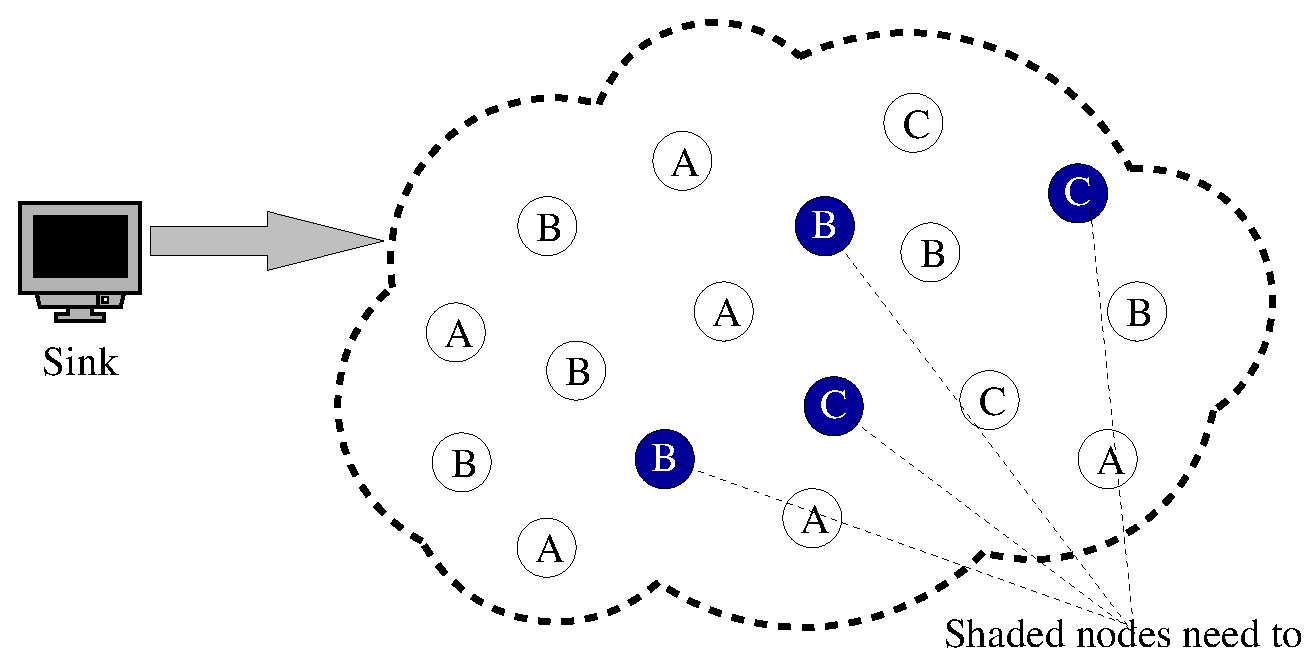
\includegraphics[scale=0.38]{figures/switch.eps}
	\caption{Software switch.}
	\label{fig:switch}
\end{figure}

Based on the above discussion, we see that both software upgrade and software switch are common and important problems in wireless sensor networks. Because the sensors are usually left unattended after deployment, such code update can only be done via wireless communication, which is an expensive operation in WSNs. For large WSNs, where the code source cannot reach the sensor node that requests the code via broadcasting, the package has to be transmitted hop-by-hop within the network, which consumes a significant amount of energy. Recent study~\cite{related:barr-energy} has shown that it consumes about the same amount of energy as executing 1000 instructions to send a single bit of data one hop away in WSN . As the sensor nodes are running with limited power supplies, it is essential to conserve the energy in a WSN during software update, especially when it happens frequently.

The goal of this research is to design an energy-efficient software update management framework for WSNs. 

\section{Challenges}

In this research, I focus on the sensor networks, that are built with low-power sensors such as the Mica2 sensors~\cite{mica2-power}. They consist of a 8 MHz ATmega128L processor, 128KB of program memory, 512KB EEPROM, 4KB of data memory, and a multi-channel radio capable of transmitting at 38.4 Kbps with an outdoor transmission range of approximately 500 feet. The device measures 2.25 inch $\times$ 1.25 inch $\times$ 0.25 inch and is typically powered by 2 AA batteries.

The major constraints of designing an energy-efficient software update management framework for such kind of sensor networks are addressed as below.

\textbf{Energy constraints}
The environment usually makes it hard to physically access the sensors after deployment, so it is difficult to replace the batteries for the sensors. Recharging the batteries using natural energy sources is not trivial, because the network might be set up in the area, such as the deep ocean, where it is hard to get access of sun light or other natural energy sources. 

Take the Mica2 sensor as an example. The energy contained in each AA battery is 15,390 Joule~\cite{battery-energy}. The experiment results in the recent study~\cite{power-tossim} showed that the energy consumption of the selected applications running on the sensors varies from 153.7 to 3,689 J/day, which makes the life time of the sensors to be 8 days to 200 days. Thus, developing an energy-efficient software update method is very important for energy limited sensor networks.


\textbf{Memory constraints}
The active program is usually stored in the program memory of a sensor node, while the other inactive programs are stored in the external flash memory. Sensor nodes will load the code image from the external flash to the program memory when they need to switch the running application from one to another.

However, due to the limited size of the flash memory, a sensor node may not be able to store the complete code images of all the applications that it needs to run. This requires the sensor nodes to download the unavailable code image from the sink node or the other neighbor nodes during {\it software switch}. How to design an energy-efficient code fetching scheme is a problem that we need to solve.

Although the sensors can fetch the wanted code image upon request, the limited sensor memory still needs to be divided wisely to store multiple code images. When the memory is not big enough to hold all the code images, an eviction scheme will be needed.

%A naive solution to this problem is to let the sensors fetch unavailable code from the sink node. However, as the observation that, different applications usually share some common code segments in MA-WSNs, the sensors can also fetch code from the nearby nodes, that have the wanted code segments. Furthermore, some sensors node, that have spare memory space, can act as external code storage node for their neighbors for fast and efficient code switch purposes.

%Now we can see that there are three roles that the memory of one sensor node is acting: storing the program code for the master sensor, storing the program code for neighboring nodes, and a message buffer during transmission. How to divide the limited memory space into the three parts is a big challenge in our software update management design.

\textbf{Network constraints}
%The wireless link in WSNs has relatively low bandwidth. As described before, Mica2~\cite{mica2-power} is equipped with a multi-channel radio capable of 38.4 Kbps bandwidth. 

The wireless links in WSNs are not stable. Both the communications and nodes are unreliable, due to the deployment environment, and the limited energy resource equipped on the sensors. The software update protocol has to be robust enough to tolerate {\em link failure} and {\em node failure} in the WSN.


\textbf{Time constraints}
Because of the high bandwidth capacity and memory usage, the sensors may not be able to perform the sensing applications during software update. So {\it software update} procedure is desired to be as fast as possible. 

\textbf{Computation constraints}
A sensor node is typically equipped with MHz (instead of GHz) micro-controller(s), which limits the complexity of  applications running on it. Therefore, the software update application that runs on the sensors have to be lightweight.



\section{Proposed software update framework}

\begin{figure}[htbp]
	\centering
		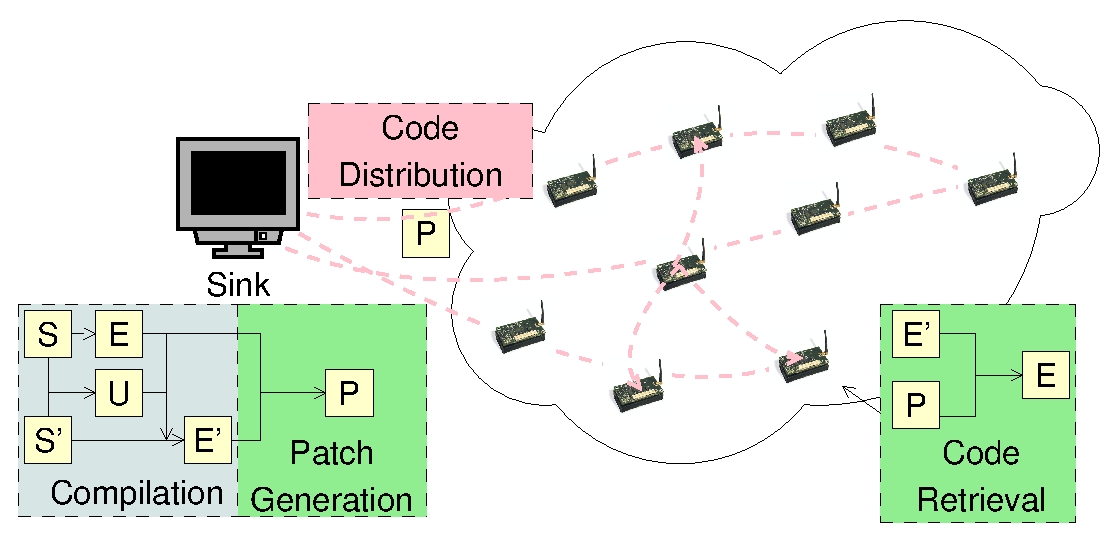
\includegraphics[scale=0.5]{figures/model.eps}
	\caption{Software update framework.}
	\label{fig:overview}
\end{figure}

In order to solve the software update problem in WSNs under all the resource constraints, I propose a software update management framework, as shown in Figure~\ref{fig:overview}. 
The sink node on the left represents a computer server, that is not resource constrained. The sensor network on the right consists of a large number of sensor nodes with resource limitations. Here, ``resource'' refers to energy, memory size,  network bandwidth, time, and CPU computation ability.

The source code is firstly translated into executable binary. Instead of sending the new binary code {\tt E'}, a smalled sized patch{ \tt P'} is distributed over the network, which only contains the differences between the new binary {\tt E'} and the binary base {\tt E}.  After code distribution is complete, the target sensor retrieves the new binary code {\tt E'} from the received patch {\tt P} and the preloaded binary base {\tt E}. 

The software update procedure includes four major steps.

%	\item {\ttControl Logic} is used by the system administrator to plan for software updates. It selects the target sensors in the network, the target software and specific version that these sensors will run later. The Control Logic also sends out the software update command, and monitor the update progress.
\textbf{Compilation} 
Because the patch transmitted over the network is the binary level difference between the base binary and the newly generated binary, increasing the binary level similarity between the newly generated binary and the base binary can reduce the number of bytes that need to be transmitted during software update. Therefore, it will save the energy consumption in software update. 
Based on this observation, I propose an update-conscious compilation technique, which uses the base binary {\tt E}, the intermediate level differences between the base version and the new version {\tt U}, as well as the new source code {\tt S}, to generate the new binary code {\tt E'}. 
	
\textbf{Patch generation}
The patch generator compares two binary versions, the base binary {\tt E} and the newly generated binary {\tt E'}. It then describes the binary code differences in a highly condensed script {\tt P}. This method reduces the size of the patch that needs to be transmitted over the network. 

\textbf{Code distribution}
The code distribution protocol disseminates the patch packets to the destination sensors that need such software update.



\section{Design goals}
The overall goal of this research is to design an efficient software update management system for WSNs. The framework is designed to solve the {\em software upgrade} problem and the {\em software switch} problem. The framework satisfies the resource constraints of WSNs, with a lower power consumption. To achieve the main goal, the following sub-goals have to be accomplished.
\begin{itemize}
	\item Design an update-conscious compilation technique, which improves the code similarity between the generated binary and  a given binary image, without too much sacrifice of the code performance. The tradeoff between the transmission power consumption in software update and the execution power consumption should be considered to guarantee overall energy savings.
	%\item Design a rapid binary code comparison scheme, which identifies the similar code structures of two binaries.
	\item Design a patch generation algorithm, which compares two code images based on their code structure, instead of bit differences. Such design has a high compression ratio, which helps to reduce the number of bytes that need to be transmitted over the network. 
	\item The code dissemination protocol should be reliable, and efficient in terms of lower power consumption and shorter distribution time. This protocol should be able to handle both {\em software upgrade}, which disseminates the code update from one source node, and {\em software upgrade}, which disseminates the target application code image from both sink and the local sensors.
\end{itemize}

\section{Assumptions}
The following assumptions are made to simplify the implementation of the software update framework in WSNs.
\begin{itemize}
\item Two software update procedures do not interleave with each other. The software update procedure always starts after the previous software update procedure is complete.
\item The sensor memory is big enough to hold both two complete code images at the same time.
\item The sensors are not preloaded with compilers, so the binary level code images have to be transmitted instead of source code.
\item Because Memory Management Unit (MMU) is not commonly equipped on the microcontroller of the sensors, the execution environment is designed to execute the binary code in the single address space. 
\item We can map the statements in both the source code level and the intermediate representation level.
\item We can estimate how many times one application will run on a sensor node.

\end{itemize}
